 % Describes how we find the peaks/clusters in the data (Maarten de Waard will
 % fill this in)
 This section will discuss how we find clusters in the raw data. 
 This is needed, to annotate these clusters, so we can later on use a
 learning algorithm on specified parts of the data.

% TODO: This piece of text is probably better suited elsewhere.
     Probably the most important of the GPS data we get from \bits are the X and Y
     position and speed of the bird. There are two speed entries in the database we
     use: One `instantaneous speed', the speed the bird has on the time of
     connecting to the GPS, calculated from two subsequent measurements, and a
     `trajectory speed', the speed the bird has between this, and the last
     measurement point. For clustering, we decided to use the latter, because this
     has a smaller error rate. Our assumption is that we can cluster the data good
     enough, by only looking at speed differences. Figure \ref{fig:speed} shows
     why.
 % TODO: Dit figuurtje maken. Ik kom er namelijk net achter dat de derivative
 % misschien niet exact doet wat we willen, omdat het speed1 en speed2 apart van
 % elkaar gebruikt. Een goeie hiervoor is device_535, sessie_000.
\begin{figure}
\centering
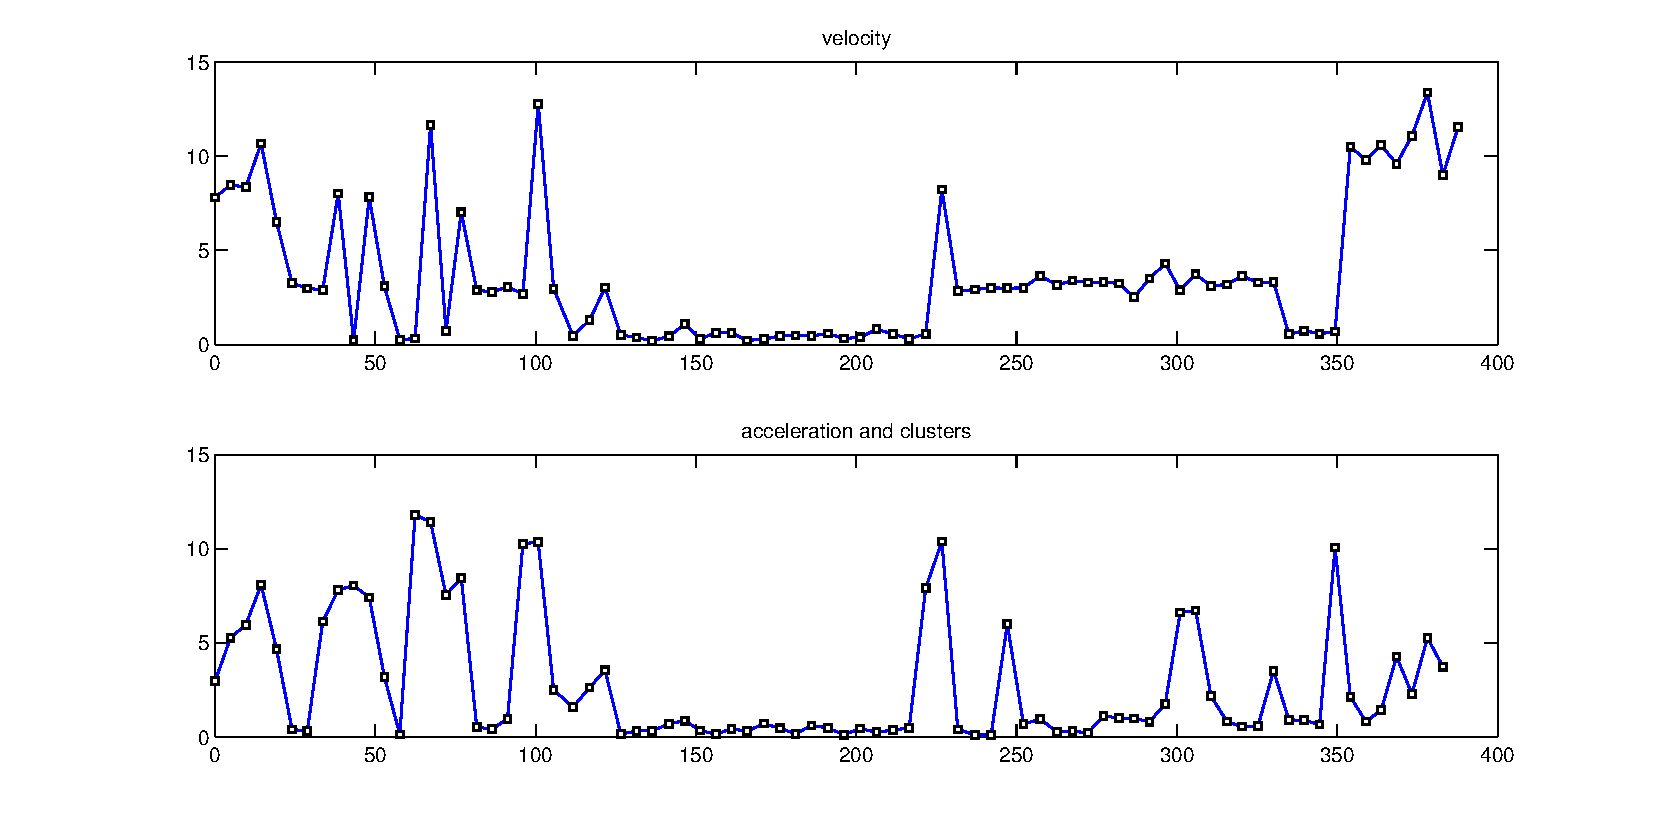
\includegraphics[width=.8\textwidth]{speed.pdf}
\caption{The speed of the bird (above) and the difference in speed (under). As
you can see, the difference is absolute (because this makes finding peaks
easier). The difference is some times a bit higher, while the speed does not
seem to differ at all. This means the bird changed his direction.}
\label{fig:speed}
\end{figure}

 As can be seen, the speed-difference is low on points where the bird is assumed
 to be flying or sitting on the water. In other points the speed differs a lot.
 On these places we can assume that the bird is foraging.

 We have tried two ways for finding clusters in the data. We started out with a
 quite straight-forward way, only looking at the speed differences of the bird.
 This worked quite well, but we needed some improvement. That is why we started
 working on a different version.

 This different version works on another basis: We create two histograms. One
 contains the trajectory speeds of the bird and the other contains the
 difference in the angle of the instantaneous speed. This means that we count
 how many times the speed or angle is between certain values, and represent that
 in an array with these counts. For further illustration see figure
 \ref{fig:histogram}.

\begin{figure}
\centering
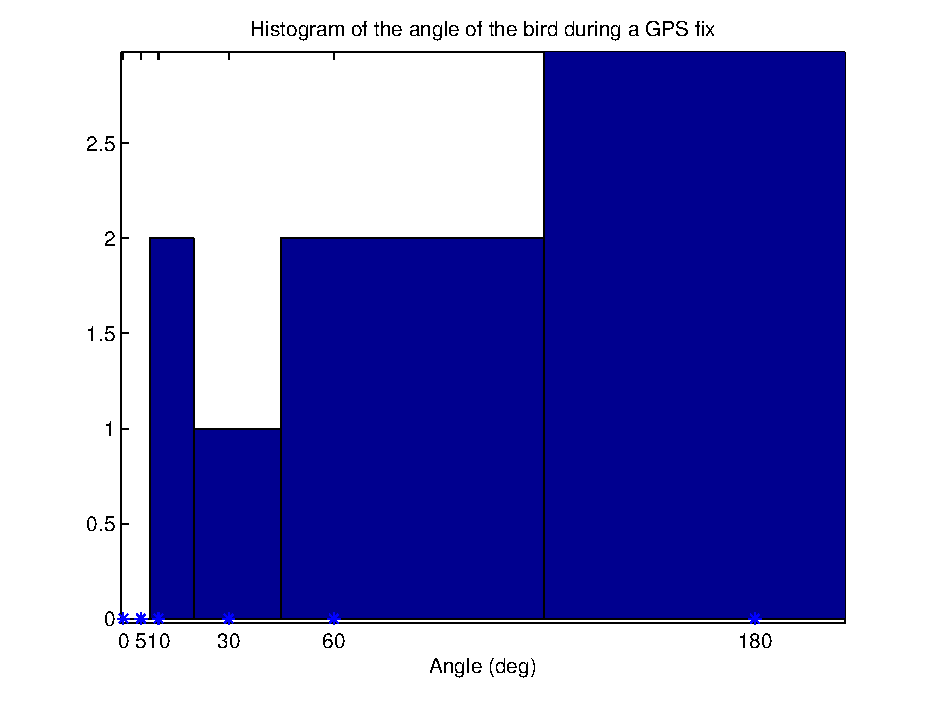
\includegraphics[width=.8\textwidth]{histogram.pdf}
\caption{Example of a histogram. The x-axis contains the bins. These are the
values in which the speeds could be. The height of the bars on the y-axis shows
us how many times in a certain time span the bird had a certain speed.}
\label{fig:histogram}
\end{figure}

\subsection{The First Way}
 \subsubsection{Finding Peaks}
 Clustering, in our case, starts with finding peaks in these speed differences.
 The peaks indicate a change in the bird's behavior, or indicate that the bird
 is foraging. Finding these peaks is done in two steps:

 \begin{itemize}
    \item Check where the value of the speed difference is bigger than a certain
    threshold.
    \item Loop through these differences and place a marker before the threshold
    is crossed upwards, or after it has been crossed downwards. 
 \end{itemize}
 
 This creates a representation of a peak by marking its left and right side.
 This comes in handy, because we do not want these speed differences in our
 clusters as they would add noise to the learning data.

 \subsubsection{Grouping Peaks}
 For grouping peaks, we created another algorithm. This algorithm looks at three
 characteristics.  
 \begin{enumerate}
 \item The time elapsed between two peaks
 \item The difference between the current time elapsed between peaks, and the
 current cluster's average
 \item The difference between the time elapsed between the first peak of the
 cluster, and the average of the rest of the cluster.
 \end{enumerate}
 This way we can find the `chaos clusters', because the time between the peaks
 in these clusters is always between a certain threshold (currently set on
 \timeThreshold seconds). 
 When a peak is too far from the  current average, this almost always indicates
 a change in behavior, so a new cluster should be started.this is done by the
 second and third characteristic specified above.

\subsection{The Second Method}
The second method we tried, relies on a bit more data. Apart from the trajectory
speed, now also the instantaneous speed is used. The trajectory speed is relevant for
the speed of the bird and now we use the instantaneous speed for finding the angle
at the time of the GPS fix. 

\begin{algorithm}
\begin{codebox}
\Procname{$\proc{histogramCompare}(Data, timeThreshold)$}
\li $exampleHists \gets getExampleHists()$
\li \For $i \gets 1 + timeThreshold$ \To $\attrib{Data}{length}$ 
\li \Do
    $currentHists \gets getHistograms(i-timeThreshold, i+timeThreshold)$
    \li $histogramValues(i) \gets \Sigma \left| currentHists - exampleHists \right|$
\End
\li \Return histogramValues
\end{codebox}
\caption{Comparing example histograms to our data}
\label{alg:hist}
\end{algorithm}

We take an example of each kind of behavior (floating, flying and foraging).
This example can be compared with a bit of the data we are
clustering. For this we loop over the data with a time window. This is probably
better explained in the pseudocode in algorithm \ref{alg:hist}.

When using this method, some problems have to be solved.

\subsubsection{Interpolating the Values}
The first problem we encounter is the difference in resolution of the data. This
would mean that when we are looking at high resolution data, and we compare it
with a low resolution example, line 4 of \ref{alg:hist} will not work. Therefore
we need to have exactly as many data points in the one, as in the other
histogram. 

This is easily achieved by interpolating the data. Since matlab has integrated
interpolation functions, we have chosen to interpolate with `Piecewise Cubic
Hermite Interpolating Polynomial (PCHIP)':, which is a bit more computationally
expensive than linear interpolation, but returns a smoother curve. This is
better, when using low resolution data, because it returns a bit smoother line.

\subsubsection{Comparing the Histograms}
As mentioned before, line 4 in algorithm \ref{alg:hist} compares two algorithms.
This returns a number close to zero, when the histograms are alike, and a high
number when they are different. Because this is not very intuitive, the program
recalculates this to percentages with equation \ref{eq:perc}.
\begin{equation}
\label{eq:perc}
percentage = 100 - \frac{Diff}{2 \sum Histogram} \times 100
\end{equation}

In this equation, Diff is the difference as calculated in algorithm
\ref{alg:hist} and the sum of a histogram is the count of all its entries. 

Now we have a percentage for each point, of how much it resembles each behavior.
A plot of this percentage is shown in the bottom of figure \ref{fig:clustering}.

\begin{figure}
\centering
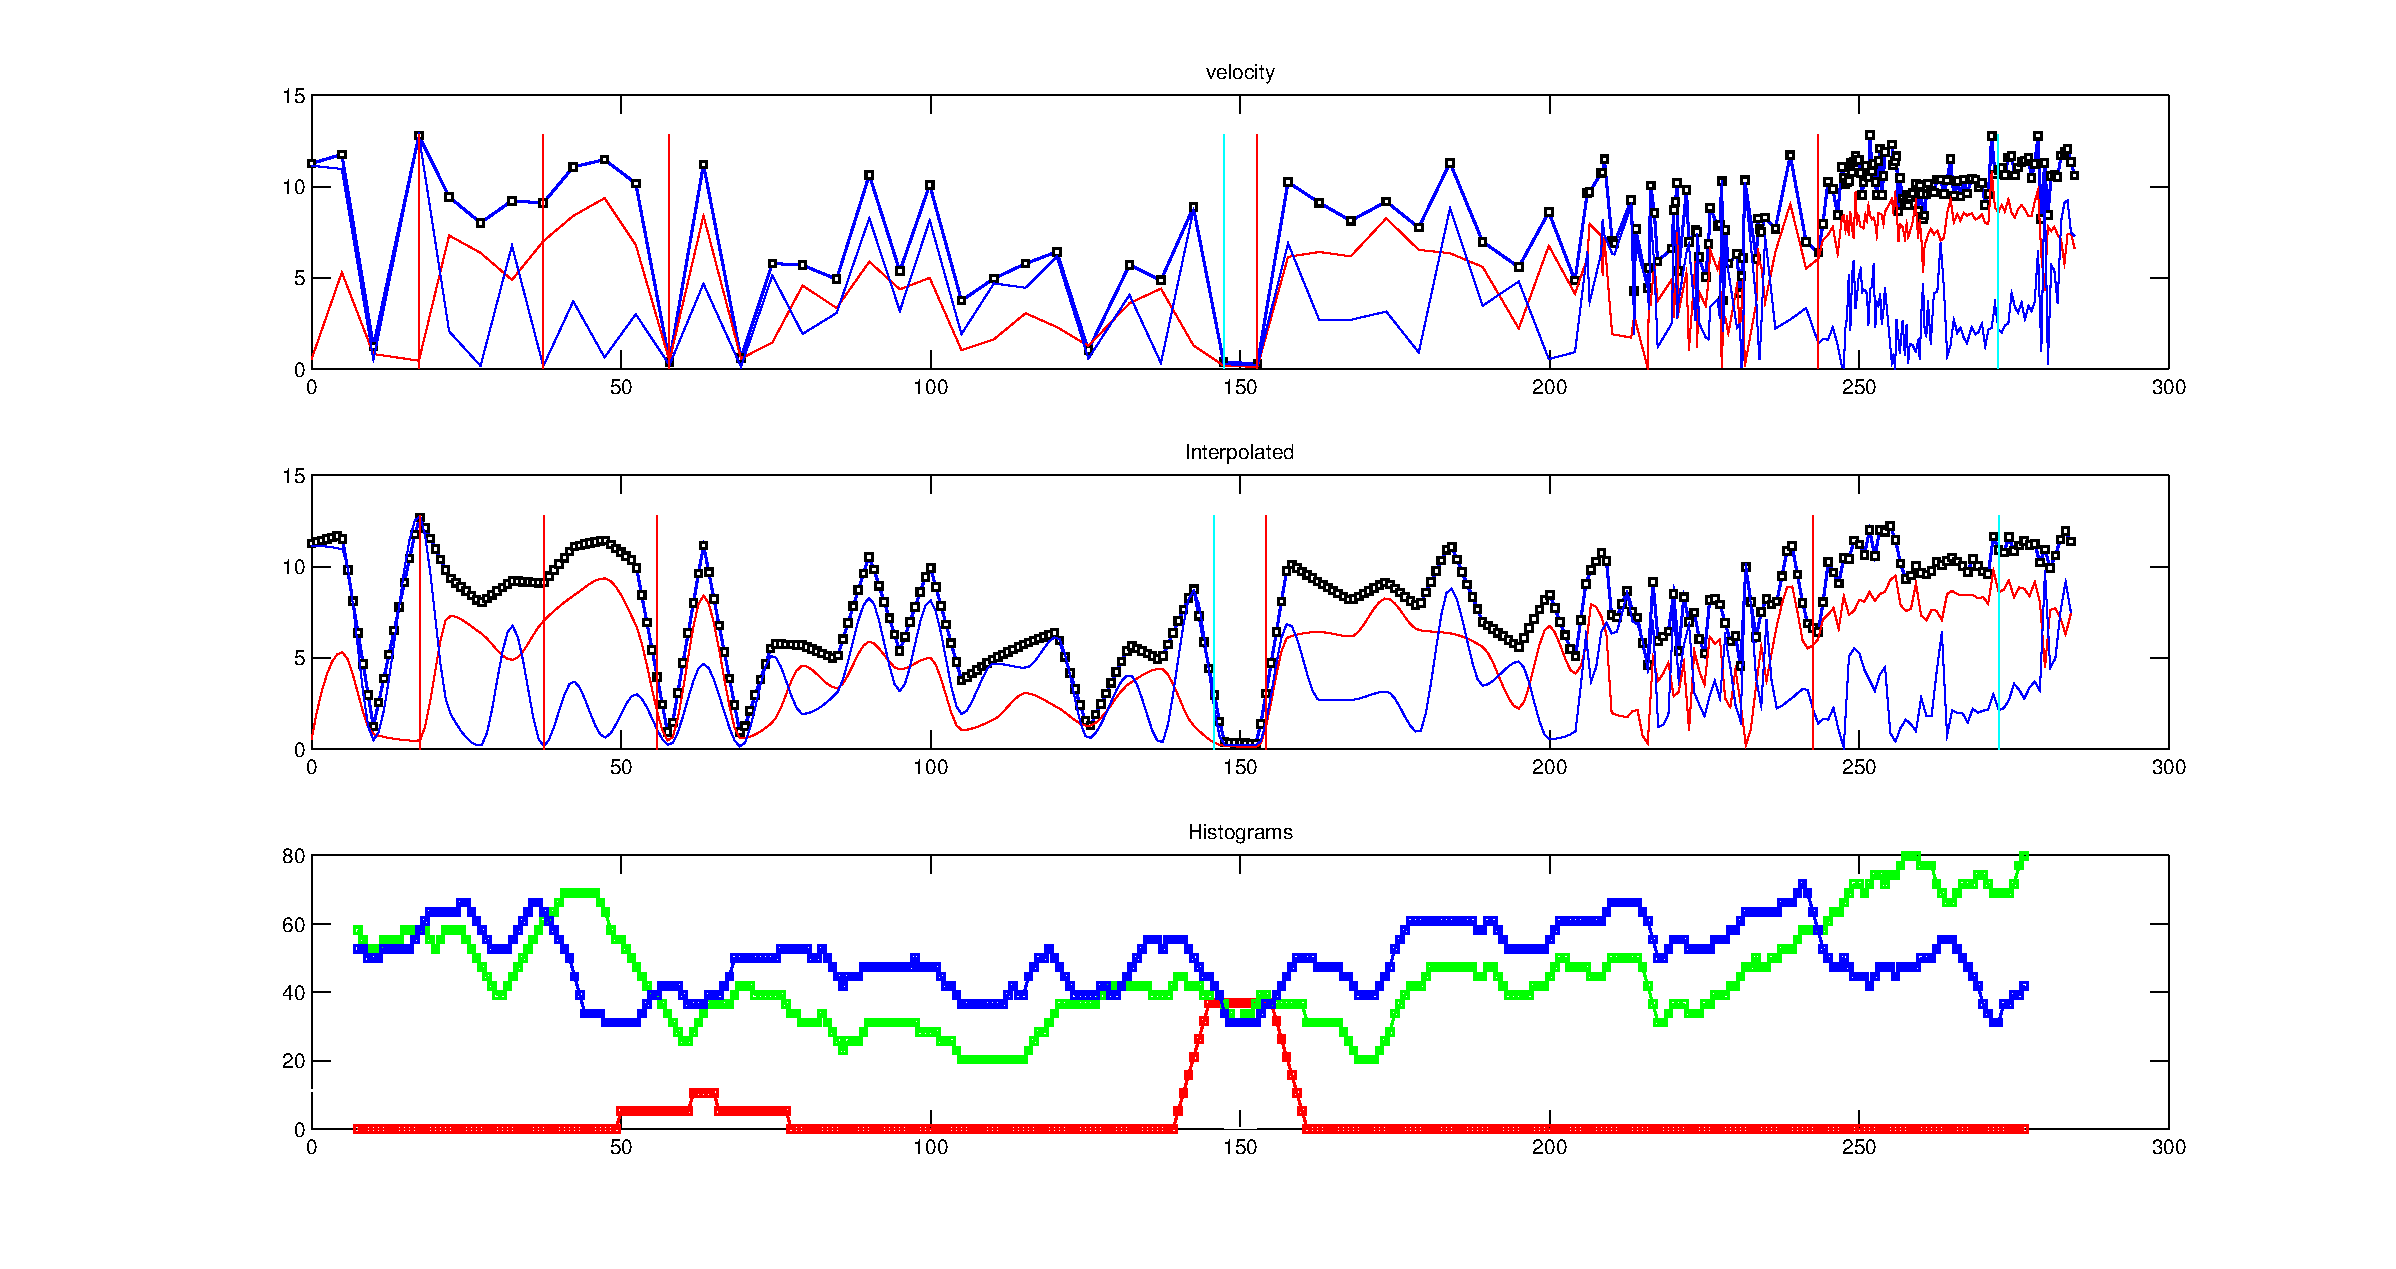
\includegraphics[width=\textwidth]{clustering.pdf}
\caption{How clustering works. Above is the raw data. The marked line is the
absolute speed of the bird. The red and blue lines under it are the speeds in
the x and y direction.
The middle image shows the interpolated data.
The bottom image shows how much the point in the middle image resembles a
certain kind of behavior. Red is floating, green is flying and blue is foraging.}
\label{fig:clustering}
\end{figure}
